% Set up the standalone document class
\documentclass{standalone}

% Input the preamble (<3)
% Preamble document

% Import tikz package
\usepackage{tikz}

% Import tikz libraries
\usetikzlibrary{shapes, arrows}
\usetikzlibrary{positioning, calc}

%----------- Create a fancy summing block
\tikzset{add/.style n args={4}{
		minimum width=6mm,
		path picture={
			\draw[black] 
			(path picture bounding box.south east) -- (path picture bounding box.north west)
			(path picture bounding box.south west) -- (path picture bounding box.north east);
			\node at ($(path picture bounding box.south)+(0,0.13)$)     {\tiny #1};
			\node at ($(path picture bounding box.west)+(0.13,0)$)      {\tiny #2};
			\node at ($(path picture bounding box.north)+(0,-0.13)$)    {\tiny #3};
			\node at ($(path picture bounding box.east)+(-0.13,0)$)     {\tiny #4};
		}
	}
}

%----------- Block style 1
\tikzstyle{block1} = [draw, fill=blue!20, rectangle, 
minimum height=3em, minimum width=6em, node distance=2.5cm]

%----------- Block style 2
\tikzstyle{block2} = [draw, fill=blue!20, rectangle, 
minimum height=3em, minimum width=3em, node distance=2.5cm]

%----------- Sum style
\tikzstyle{sum} = [draw, fill=blue!20, circle, node distance=2cm]

%----------- Input style
\tikzstyle{input} = [coordinate, node distance=4cm]

%----------- Output style
\tikzstyle{output} = [coordinate, node distance=4cm]

%----------- Pin style
\tikzstyle{pinstyle} = [pin edge={to-,thin,black}]

\begin{document}
	
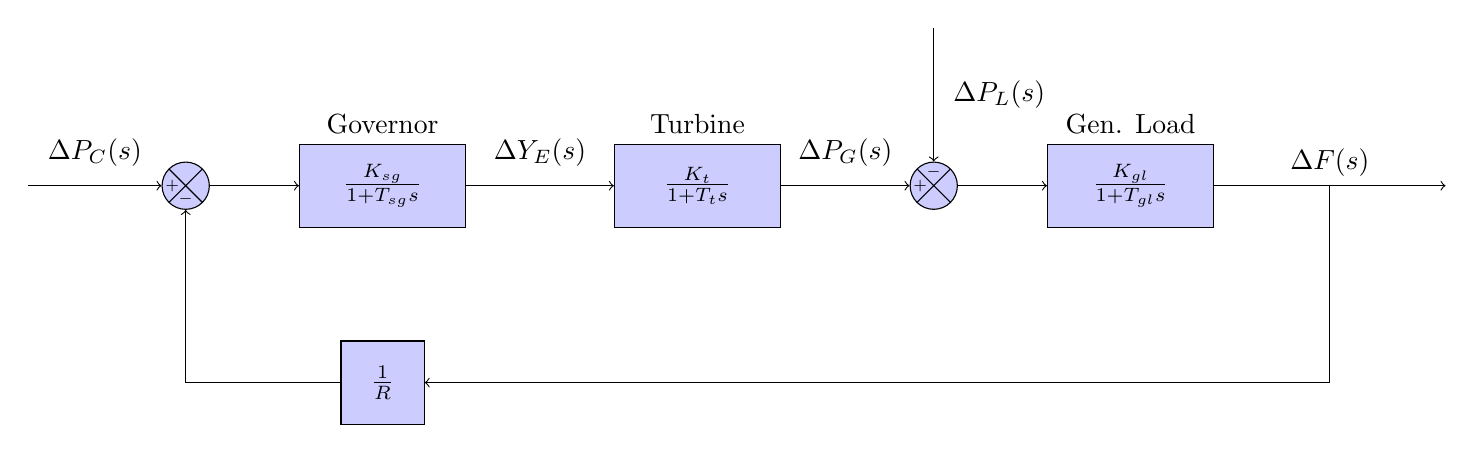
\begin{tikzpicture}
	
	% Draw the nodes first
	\node [input] (input) {};
	\node [sum, add={$-$}{+}{ }{ }, right of=input] (sum1) {};
	\node [block1, right of=sum1, label=above:{Governor}] (governor) {$\frac{K_{sg}}{1 + T_{sg}s}$};
	\node [block2, below of=governor] (regulator) {$\frac{1}{R}$};
	\node [block1, right of=governor, label=above:{Turbine}, node distance=4cm] (turbine) {$\frac{K_t}{1 + T_t s}$};
	\node [sum, add={ }{+}{$-$}{ }, right of=turbine, node distance=3cm] (sum2) {};
	\node [input, above of=sum2, node distance=2cm] (demand) {};
	\node [block1, right of=sum2, label=above:{Gen. Load}] (genload) {$\frac{K_{gl}}{1 + T_{gl}s}$};
	\node [output, right of=genload] (output) {};
	
	% Connect the nodes
	\draw [->] (input) -- node [label=above:{$\Delta P_C(s)$}] {} (sum1);
	\draw [->] (sum1) -- (governor);
	\draw [->] (governor) -- node [label=above:{$\Delta Y_E(s)$}] {} (turbine);
	\draw [->] (turbine) -- node [label=above:{$\Delta P_G(s)$}] {} (sum2);
	\draw [->] (demand) -- node [label=right:{$\Delta P_L(s)$}] {} (sum2);
	\draw [->] (sum2) -- (genload);
	\draw [->] (genload) -- node [coordinate, name=feedback, label=above:{$\Delta F(s)$}] {} (output);
	\draw [->] (feedback) |- (regulator);
	\draw [->] (regulator) -| (sum1);
	
\end{tikzpicture}
	
\end{document}